% =========================================================
%  Cabeçalho
% =========================================================

% Define papel, tamanho global de fonte, tipo de documento
\documentclass[a4paper, twoside, 12pt]{article}

% Pacotes usados
\usepackage[utf8]{inputenc} % enconding de caracteres
\usepackage[brazil]{babel}  % locale pt_BR
\usepackage[lmargin=2cm, rmargin=2cm, tmargin=2cm, bmargin=2cm]{geometry} % margens da folha
\usepackage{indentfirst} % sempre indenta o primeiro parágrafo

% Multicolunas
\usepackage{multicol}

% Matemática
\usepackage{amsmath}
\usepackage{amsfonts}
\usepackage{gensymb}

% Tabela longa que quebra entre as paginas
\usepackage{longtable}

% Para links e url
\usepackage[hidelinks]{hyperref}

% Código fonte
\usepackage{listings} % listagem de código-fonte
\renewcommand*{\lstlistingname}{Listagem} % texto para listagem de código
\usepackage{color} % cor para usar na listagem de código-fonte

% Imagens
%\usepackage{svg}
\usepackage{graphicx,xcolor} % para inserir imagens
\usepackage[nottoc,notlot,notlof]{tocbibind} % adiciona o tópico Referências ao Sumário
\usepackage{textcomp} % accesso \textquotesingle

% Para desenhar grafos
\usepackage{tikz}
\usetikzlibrary{arrows,positioning,shapes,decorations}

% Desenhar circulos
%\usepackage{tkz-euclide}
%\usetkzobj{all}

% Escrever algoritmos em pseudo-código
%\usepackage[portuguese,linesnumbered]{algorithm2e}

% Tabelas
\usepackage{booktabs}
\usepackage{caption}

% Estilos para usar nos grafos
\tikzset{
	>=stealth',
	punkt/.style={
		rectangle,
		text centered,
		inner sep=0.7em,
		draw,
		fill=blue!5
	},
	pil/.style={
		->,
		thick,
		shorten <=2pt,
		shorten >=2pt
	}
}

% Para plotar gráficos
%\usepackage{pgfplots}
%\pgfplotsset{width=10cm,compat=1.9}

% Define cores para o highlight de código-fonte
\definecolor{dkgreen}{rgb}{0,0.6,0}
\definecolor{gray}{rgb}{0.5,0.5,0.5}
\definecolor{mauve}{rgb}{0.58,0,0.82}

% Define configuração para listagem de código-fonte em linguagem C
\lstset{
	frame=tb,
	language=C,
	aboveskip=2mm,
	belowskip=2mm,
	showstringspaces=false,
	columns=flexible,
	basicstyle={\small\ttfamily},
	numbers=none,
	keywordstyle=\color{blue},
	commentstyle=\color{dkgreen},
	stringstyle=\color{mauve},
	breaklines=true,
	breakatwhitespace=false,
	tabsize=4
}

% =========================================================
%  Documento
% =========================================================

% Começo do documento
\begin{document}

% Define algum espaçamento que eu não lembro, hehe :)
\setlength\parskip{0.3cm}

% =========================================================
%  Capa
% =========================================================

% Começo da folha de Capa
\begin{titlepage}

		% Título
		\title{
\textsc {\large{Universidade de São Paulo\\
Instituto de Ciências Matemáticas e de Computação}}\\[1cm]
\large{SCC0217 -- Linguagens de Programação e Compiladores}\\[6cm]
\LARGE{Trabalho 4 -- Paradigma de Programação Funcional}\\[5.5cm]
		}

		% Autores
		\author{
Elias Italiano Rodrigues -- 7987251\\
Vinicius Katata Biondo -- 6783972
		}

		% Inserção manual de data
		\date{
\vfill São Carlos, 20 de maio de 2015
		}

		% Cria a Capa
		\maketitle
		\thispagestyle{empty}

% Fim da folha de Capa
\end{titlepage}
	
% Reseta contador de página para 1 (assim não conta a Capa como página)
\setcounter{page}{1}

% =========================================================
%  Sumário
% =========================================================

% Cria o Sumário
\tableofcontents

% Cria uma nova página, forçando o Sumário a ficar numa página separada
\clearpage

% =========================================================
%  Conteúdo
% =========================================================

\section{Introdução \label{sec:introducao}}

Este é um trabalho de pesquisa sobre o paradigma de programação funcional. Junto a este documento, acompanha um conjunto de \textit{slides} de apresentação. O conteúdo deste trabalho é baseado no capítulo 15 ``\textit{Functional Programming Languages}" do livro-texto \cite{bib:livro} da disciplina relacionado a linguagens de programação.

\subsection{O Paradigma}

O paradigma de programação funcional, que é baseado em funções matemáticas, é a base de projeto de uma das mais importantes linguagens não-imperativas: LISP.

Segundo John Backus (1978), linguagens de programação puramente funcionais são melhores que linguagens imperativas, porque elas resultam em programas mais legíveis, confiáveis e mais propensos a não conter erros; devido a serem mais fáceis de se entender principalmente por causa do significado das expressões serem independentes do seu contexto -- não possui efeitos colaterais ou mudanças de estado durante a execução do programa.

LISP começou como uma linguagem puramente funcional, mas logo adquiriu algumas das importantes características das linguagens imperativas que aumentaram seu desempenho durante a execução. Ainda hoje, é uma das mais importantes linguagens funcionais com uso nas áreas de aprendizado de máquina, representação de conhecimento e sistemas inteligentes.

\subsection{Funções Matemáticas}

Uma função matemática é o mapeamento de elementos de um conjunto (domínio) em outro conjunto (contra-domínio). Esse mapeamento é geralmente descrito como uma expressão. Funções se aplicam a elementos particulares do domínio, que são informados como parâmetros, e o seu resultado é um elemento do contra-domínio.

Uma das características fundamentais das funções matemáticas é que a avaliação das expressões de mapeamento são controladas por recursão e expressões condicionais, ao invés do sequenciamento e iteração que são comuns nas linguagens de programação imperativas. Outra característica importante é que elas não dependem de valores externos e portanto não tem efeitos colaterais. Um parâmetro de uma função matemática assume um único valor quando está sendo avaliada, ou seja, seu valor não altera durante a execução da função, diferentemente dos parâmetros nas principais linguagens de programação.

Em um programa imperativo, uma função pode ter dependência de valores de variáveis locais ou globais. Isso torna difícil de determinar os valores que serão produzidos no final da execução.

Em matemática, não existem variáveis que modelam alocação de memória nem que guardam o estado da função matemática. Uma função matemática mapeia seus parâmetros em valores ao invés de especificar uma sequência de operações sobre valores em uma memória para produzir um resultado.

\subsection{\textit{Lambda Calculus}}

Notação \textit{lambda} foi idealizada por Alonzo Church, em 1941, que forneceu uma forma de descrever funções independente do nome, isto é, as funções são especificadas apenas pelos parâmetros  e pela expressão da função, por exemplo:

\indent\indent		$\lambda$(x) x*x*x

Além disso, Church também definiu formalmente sistemas para definição e aplicação de funções e recursão usando expressão \textit{lambda}. Esses sistemas são conhecidos como \textit{Lambda Calculus}, que serve de inspiração para linguagens de programação funcional.

As expressões \textit{lambda} mantêm as características de funções matemáticas, os parâmetros podem assumir qualquer valor do domínio, antes da avaliação da função, pois durante, assume um único e inalterável valor. É importante notar que as expressões \textit{lambda} aceitam mais de um parâmetro assim como funções matemáticas.

\section{Noções Básicas \label{sec:nocoes-basicas}}

O objetivo do projeto de uma linguagem de programação funcional é o de imitar funções matemáticas o máximo possível o que resulta numa abordagem de resolução de problemas fundamentalmente diferente da abordagem com linguagens imperativas. Em uma linguagem imperativa, uma expressão é avaliada e seu resultado é armazenado em uma posição de memória, que é representado por uma variável no programa. Essa atenção às posições de memória, que representam os estados do programa, resulta numa metodologia de programação de baixo-nível.

Uma linguagem puramente funcional não usa variáveis ou atribuições livrando assim o programador de preocupações relacionadas às posições de memória ou estado do programa. Sem o uso de variáveis, construções iterativas não são possíveis pois elas são controladas por variáveis, logo, repetição deve ser especificada como recursão.

Sem variáveis, em uma execução puramente funcional, não há estados. A execução sempre produz os mesmos resultados quando informados os mesmos parâmetros. Essa característica chama-se transparência referencial. Além de tornar a semântica mais simples, esta característica também torna os testes mais fáceis, pois cada função pode ser testada separadamente sem preocupações com o contexto.

Uma linguagem funcional provê um conjunto de funções primitivas, um conjunto de formas funcionais para construir funções complexas a partir das primitivas, uma operação de aplicação de função e estruturas para representar os dados.

\clearpage
\section{Linguagens \label{sec:linguagens}}

Atualmente muitas linguagens funcionais foram desenvolvidas, porém algumas tomaram um rumo mais parecido com as linguagens imperativas adquirindo algumas ferramentas que aumentam a eficiência de execução. LISP é um exemplo.

Outras linguagens como ML e Haskell conduziram um expansão considerável em certas áreas da computação onde elas são utilizadas. Essas linguagens cresceram assim como a sua utilização. Hoje em dia são usadas em diversas áreas como processamento em banco de dados, modelos financeiros, análises estatísticas, bio-informática, e algumas outras áreas.

ML é uma linguagens baseada em fundamentos funcionais, porém muitas vezes é dita impura, pois permite efeitos colaterais o que é negado nas linguagens puramente funcionais. Muitas novas linguagens surgiram a partir de ML, essas são chamadas de família ML, as mais conhecidas são SML, Caml e F\#. Além disso, influenciou a criação de novas linguagens como Haskell.

Nos próximos capítulos, será discutido mais detalhadamente sobre as linguagens LISP e Haskell.

\section{LISP \label{sec:lisp}}

LISP é a mais antiga e usada linguagem de programação funcional. Foi desenvolvida por John McCarthy no MIT em 1959. Ao longo do tempo, adquiriu algumas características de linguagens imperativas como variáveis no estilo imperativo (que representam uma região de memória que pode ter valor alterado várias vezes), atribuições e iteração. Apesar disso, LISP ainda representa bem os conceitos fundamentais de programação funcional.

\subsection{Listas}

Existem somente dois tipos de objetos de dados no LISP: átomos e listas. Elementos de uma lista são compostos por duas partes: a primeira é o dado do elemento, o qual pode ser um ponteiro para um átomo ou para uma lista aninhada. A segunda parte pode ser um ponteiro para um átomo, um ponteiro para outro elemento ou uma lista vazia. Esses elementos, átomos e listas, não contém um tipo de dado, como nas linguagens imperativas.

Listas são declaradas delimitando seus elementos com parêntesis, como o exemplo a seguir:

\begin{verbatim}
    (A B C D)
\end{verbatim}

Listas aninhadas também são delimitadas por parêntesis:

\begin{verbatim}
    (A (B C) D (E (F G)))
\end{verbatim}

Neste último exemplo, a lista contém quatro elementos, sendo eles \texttt{A}, \texttt{(B C)}, \texttt{D} e \texttt{(E (F G)))}.

\clearpage
\bigskip 
\begin{center}
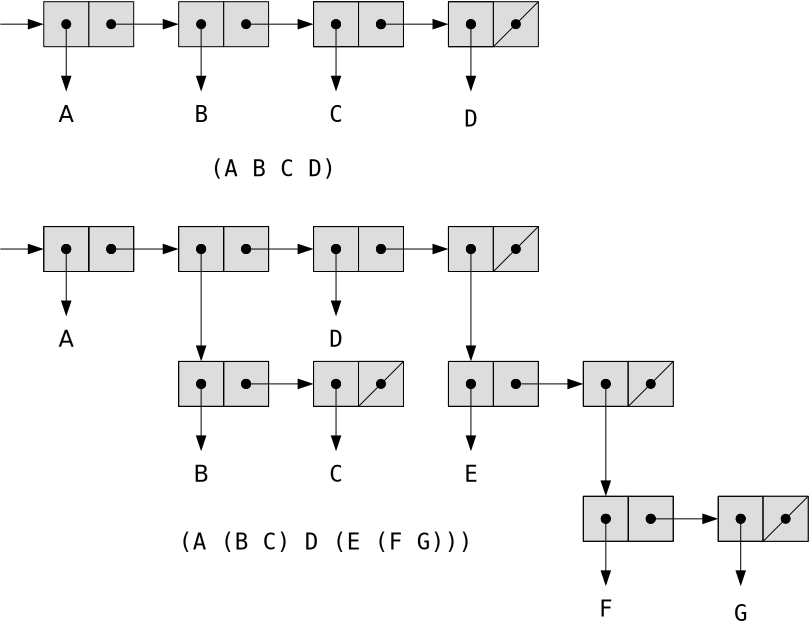
\includegraphics[scale=0.50]{../listas.pdf}
% inkscape -D -z --file=listas.svg --export-pdf=listas.pdf
\end{center}

Uma lista é guardada como uma lista encadeada na qual cada nó tem dois ponteiros, um para referenciar o dado do nó e outro para formar a lista ligada. A lista é referenciada pelo ponteiro do seu primeiro elemento.

A partir do conceito de processamento de listas ser uma maneira de estudar a computabilidade de problemas, que até então era feito através de máquinas de Turing, surgiu a ideia de se construir uma função LISP universal com capacidade de avaliar outra função LISP. Logo o primeiro requisito para essa função universal era que sua estrutura fosse expressada semelhante aos dados. Como a forma de parêntesis já tinha sido adotada para os dados, inventou-se convenções para definição de funções e chamada de funções na mesma forma, para que assim as funções conseguissem ser expressas na forma de listas.

A expressão \textit{lambda} que foi escolhida para definição de funções teve de ser modificada para aceitar que uma função seja vinculada a um nome, para que depois esta possa ser referenciada por outras funções ou até mesmo por ela mesma.

\subsection{Funções Primitivas}

Funções do LISP podem ser divididas em duas classes: as funções primitivas e as funções definidas pelo usuário. Funções primitivas são funções que o LISP já conhece, ou seja, nativas. Existem primitivas que operam sobre números, símbolos e listas.

As funções primitivas que operam sobre números são as operações algébricas básicas como adição, subtração, multiplicação e divisão. Além dessas, também é reconhecida como uma primitiva a função de raiz quadrada. O padrão para chamada de uma função em LISP é o seguinte:

\begin{verbatim}
    (FUNCTION INPUT)
\end{verbatim}

A operação de multiplicação e adição aceitam zero ou mais parâmetros, caso o número de parâmetros seja zero em ambos os casos, o elementos neutro é retornado. Já na subtração e divisão são aceitos no mínimo dois parâmetros. Na subtração todos números, exceto o primeiro, são subtraídos do primeiro elemento, analogamente para a divisão. Alguns exemplos dessas           funções:

\begin{verbatim}
    (/ 23 8.0)
    2.875
\end{verbatim}

\begin{verbatim}
    (- 7 6 5)	
    -4
\end{verbatim}

\begin{verbatim}
    (+ 3 5.6)
    8.6
\end{verbatim}

	As funções podem ser aninhadas e são tratadas dos parêntesis mais internos até exteriores:
	
\begin{verbatim}
    (+ 3 (- 3 2))
    4
\end{verbatim}

Além das funções algébricas básicas, existem também outras primitivas como \texttt{ABS}, \texttt{ROUND}, \texttt{FLOAT}, \texttt{LENGTH}, \texttt{FIRST}, \texttt{REST}, \texttt{LAST}, \texttt{APPEND}, \texttt{CONS}, \texttt{LIST}, \texttt{RANDOM}, \texttt{COND}. Outra primitiva muito importante em LISP é a aspa simples, pois é possível fazer com que o primeiro elemento de uma lista não seja avaliado como uma função, isso evita que um símbolo seja confundido com um nome de uma função.
	
Não vem ao caso especificar cada uma dessas funções, porém elas mantém um nome bem sugestivo ao seu uso.

\subsection{Predicados}

Predicados são funções primitivas que retornam verdadeiro  ou falso. Verdadeiro em LISP é representado pelo símbolo \texttt{T} e falso é representado por \texttt{NIL}. Um exemplo bem simples de predicado é \texttt{SYMBOLP}, que retorna \texttt{T} se o dado de entrada é um símbolo e falso caso contrário.

\begin{verbatim}
    (symbolp nil)
    T
\end{verbatim}	

\begin{verbatim}
    (symbolp .435)
    NIL
\end{verbatim}

Existem também a função \texttt{NUMBERP} que retorna \texttt{T} caso o dado passado seja um número, se não retorna \texttt{NIL}. Assim como esses, existem vários outros predicados para checar se o dado entrado é de um certo tipo \texttt{FLOATP}, \texttt{INTEGERP}, \texttt{ODDP} e \texttt{EVENP}.

Outros predicados muito utilizados em LISP são os operadores relacionais como \texttt{<}, \texttt{>}, \texttt{<=}, \texttt{>=}, \texttt{=} e \texttt{/=} que comparam dois números e retorna o resultado.

\begin{verbatim}
    (< 67 34.5)
    NIL
\end{verbatim}

\begin{verbatim}
    (>= 76 68)
    T
\end{verbatim}

\begin{verbatim}
    (= 67 67 90 67 67)
    NIL
\end{verbatim}

\begin{verbatim}
    (/= 4 5)
    T
\end{verbatim}

Pode-se checar se um número é maior ou menor que zero utilizando funções predicados específicos chamados \texttt{PLUSP} e \texttt{MINUSP}, respectivamente. Além disso, podemos comparar strings utilizando a função \texttt{EQUAL}, uso é análogo às outras.

Assim como nas funções primitivas, além das citadas existem muitos outros predicados, porém não é conveniente a citação de todos nesse trabalho.

\subsection{Estruturas de Controle}

LISP provê duas formas de controlar e organizar o fluxo de execução de um programa, uma dessas maneiras é através de funções condicionais e outra é aplicando recursão em funções. É possível encontrar no Common LISP, \texttt{IF} e \texttt{CASE}, onde a primeira só é possível fazer uma escolha de dois caminhos, já na segunda função mais opções de caminhos são possíveis. Inúmeras outras formas iterativas de controle como \texttt{FOR}, \texttt{DO} e \texttt{WHILE} podem ser encontradas no Common LISP.

A expressão condicional \texttt{COND} é uma das primitivas do LISP e é da seguinte forma:

\begin{verbatim}
    (cond
        ( <teste 1> <s-expr> <s-expr> . . . <s-expr> <resultado 1> ) 
        ( <teste 2> <s-expr> <s-expr> . . . <s-expr> <resultado 2> ) 
        .
        .
        .
        ( <teste n> <s-expr> <s-expr> . . . <s-expr> <resultado n> ) 
    )
\end{verbatim}

Avaliação dessa expressão é feita da seguinte maneira.

O primeiro elemento da primeira cláusula é testado (\texttt{<teste 1>}), caso seja verdade todos os outros elementos (\texttt{<s-expr>}) da primeira cláusula são avaliados e a avaliação do elemento final (\texttt{<resultado 1>}) é retornado como valor da expressão \texttt{COND}. As outras cláusulas são ignoradas. Caso a avaliação do primeiro elemento da primeira cláusula seja \texttt{NIL} todo o resto dessa parte é ignorado, logo a segunda cláusula é testada. E isso continua até que a expressão retorna um valor ou \texttt{NIL}.

A segunda forma que se pode controlar o fluxo de um programa é fazer uma chamada recursiva de função, um exemplo para isso seria a função abaixo que retorna o n-ésimo termo de uma lista:

\begin{verbatim}
    (defun list-nth (n L)
        (cond
            ((null L) nil)
            ((zerop n) (first L))
            (t (list-nth (1- n) (rest L)))
        )
    )
\end{verbatim}

\subsection{Exemplos}

O programa ``Hello, world!":

\begin{verbatim}
    (print "Hello, world!")
\end{verbatim}

Programa fatorial:

\begin{verbatim}
    (defun factorial (n)
        (if (= n 0) 1
            (* n (factorial (- n 1)))
        )
     )
\end{verbatim}

\section{Haskell \label{sec:haskell}}

Haskell (Thompson, 1999) é uma linguagem de programação puramente funcional, ou seja, não possui expressões ou declarações que tem efeitos colaterais.

O seguinte código define uma função fatorial em Haskell:

\begin{verbatim}
    fact 0 = 1
    fact 1 = 1
    fact n = n * fact(n - 1)
\end{verbatim}

Linhas podem ser adicionadas para especificar as circunstâncias sob a qual a definição deve ser aplicada. Por exemplo:

\begin{verbatim}
    fact n
        | n == 0 = 1
        | n == 1 = 1
        | n > 1  = n * fact(n - 1)
\end{verbatim}

\clearpage
\section{Conclusão \label{sec:conclusao}}

Neste trabalho foi apresentado o paradigma de programação funcional. A realização deste trabalho possibilitou momentos de pesquisa e contato com a especificação de paradigmas de linguagens de programação assim como é exposto no livro-texto.

Através de uma revisão bibliográfica, foi possível concluir que apesar de esforços para manter uma linguagem puramente funcional, quando é sentido a necessidade de uma otimização desse paradigma é necessário apelar para o modo de funcionamento das linguagens tradicionais.

% =========================================================
%  Referências
% =========================================================

\clearpage % força criar uma nova página

% Começo das Referências
\begin{thebibliography}{9}

	\bibitem{bib:livro}
		SEBESTA, Robert W. \textit{Concepts of Programming Languages}. United States of America: Pearson, 10ed., 2010.

% Fim das Referências
\end{thebibliography}

% Fim do documento
\end{document}
